% ============================================================================================================
\chapter{Audit de la version 0.7}\label{ch:audit}
% ============================================================================================================

L'audit reprend les six limites identifiées à la fin de la phase 3 et cherche, pour chacune, le mécanisme réellement
implémenté, ses hypothèses implicites, ses conséquences, la nature du problème (conceptuel, statistique,
informatique ou de données) et plusieurs corrections possibles. Le détail est dans \code{doc/18\_audit\_v07\_phase31.md}.

\section{Un défaut de code découvert en cours d'audit}

\begin{limites}[Défaut de la v0.7]
Dans la fonction qui résout chaque année du modèle, un paramètre nommé \code{amorti} règle l'amortissement de la
résolution itérative (0,5). En v0.7, la nouvelle fermeture utilisait une variable du même nom pour son terme
proportionnel (0,3), qui écrasait donc l'amortissement de la résolution. Quand la résolution converge, le résultat est
le même ; mais les essais de la v0.7 avec un terme proportionnel nul arrêtaient la résolution, et l'« instabilité »
qui avait fait retenir 0,3 était un artefact. Le défaut est corrigé, un test empêche sa réapparition, et tous les
résultats de la v0.7 ont été recalculés.
\end{limites}

Ce défaut explique en partie les oscillations de période deux ans observées en v0.7. Les réponses impulsionnelles
recalculées montrent que deux termes en différence, ajoutés sans estimation en v0.7 (le terme proportionnel de la
fermeture et l'effet des tensions de capacité sur les importations), produisent aussi ces oscillations, que les
écarts de production observés ne présentent pas.

\section{Les six limites}

\begin{table}[htbp]\centering\scriptsize
\caption{Synthèse de l'audit de la v0.7.}\label{tab:audit}
\begin{tabularx}{\linewidth}{@{}p{3.2cm}LLl L@{}}\toprule
Limite & Mécanisme v0.7 & Conséquence & Nature & Correction retenue\\ \midrule
Distribution statique & Microsimulation avant/après la mesure, revenus de l'année de base & Gagnants mal mesurés ; prélèvements sur les entreprises sans perdants & Conceptuelle, données & Distribution dynamique hybride (M16)\\
Transmission demande-potentiel & θ = 1,5 choisi par simulation & Dette de S3 en 2047 de $-9$ à +43 points & Statistique & Estimation par la durée des écarts de production ; θ = 0,75 (0,5-1,0)\\
Pas de backtest & Rétrosimulations courtes de la v0.6 & Pas de mesure des erreurs du modèle complet & Informatique, données & Rétrosimulations en temps réel 2010-2019 et 2021-2025\\
Cinq cas types & Offre de travail sur 5 configurations & Effets mal répartis (logement, nombre d'enfants) & Calcul & 18 cas types\\
Incidence fiscale & Profits et prix seulement & IS, impôts de production indolores pour les salariés & Conceptuelle, empirique & Incidence salariale de long terme, fourchettes de la littérature\\
Comportements d'entreprises & Paramètres de la littérature, non estimés & Résultats fragiles sur l'offre & Empirique & Confrontation aux évaluations ; maintien en exploratoire\\ \bottomrule
\end{tabularx}
\end{table}

\section{Options étudiées pour la distribution}

Trois approches ont été comparées. Une microsimulation dynamique complète (transitions individuelles entre emploi et
chômage, vieillissement) est la plus rigoureuse, mais suppose des transitions estimées sur un panel qui n'est pas en
données ouvertes. Une population synthétique par cellules (décile × statut × famille) est légère, mais perd
l'hétérogénéité au sein des cellules. L'approche retenue est hybride : les 41 000 ménages pondérés de la
microsimulation conservent leurs caractéristiques ; chaque effet macroéconomique leur est appliqué selon leur
exposition ; les effets d'emploi sont calculés en espérance ; la somme est confrontée au revenu disponible du modèle
macroéconomique.

% ============================================================================================================
\chapter{Corrections apportées}\label{ch:corrections}
% ============================================================================================================

\begin{enumerate}
\item \textbf{Défaut de code} : corrigé (variable renommée), test de non-régression.
\item \textbf{Fermeture} : suppression des deux termes en différence non estimés ; ρ et θ estimés (chapitre~\ref{ch:equations}).
\item \textbf{Référence} : recalée avec la nouvelle fermeture ; l'ancienne fermeture (sur le chômage) et la nouvelle
donnent exactement la même trajectoire de référence (écart maximal de chômage $10^{-5}$ point).
\item \textbf{Incidence fiscale} : part de l'IS, des impôts de production et des cotisations employeurs supportée à
long terme par les salariés, via la cible de long terme du coût salarial.
\item \textbf{Distribution dynamique} : nouveau module M16.
\item \textbf{Offre de travail} : 18 cas types au lieu de 5.
\item \textbf{Simulateur} : niveaux de paramètres par famille (offre de travail, incidence, assurance chômage, R\&D,
formation) et surcharges individuelles, pour l'analyse de sensibilité un à un ; la référence est désormais recalculée
dès qu'un paramètre de fermeture change (en v0.7, une variante de ρ était comparée à une référence calculée avec
la valeur centrale : défaut corrigé).
\end{enumerate}

Ce qui n'a pas été modifié, et pourquoi : les équations estimées (consommation, investissement, commerce, emploi,
salaires, prix) restent celles de la v0.6, déjà testées hors échantillon ; le comportement des entreprises par taille
reste non représenté faute de données ouvertes suffisantes à l'échelle du modèle ; la convention « autres dépenses
proportionnelles au PIB nominal » est conservée.

% ============================================================================================================
\chapter{Modèles et équations retenus}\label{ch:equations}
% ============================================================================================================

\section{Fermeture}

\begin{equation}
Z_t = Z_{t-1} - \rho\, g_{t-1} + \theta\,(\ln Y^*_{t-1}-\ln Y^{*,\mathrm{ref}}_{t-1}), \qquad g_t = \ln Y_t - \ln Y^*_t,
\end{equation}
avec ρ = 0,2 et θ = 0,75. $Z$ est un supplément de demande intérieure (60 \% consommation, 40 \% investissement) qui
représente les canaux non modélisés de retour vers le potentiel ; θ représente l'anticipation, par les ménages et les
entreprises, d'une révision durable du potentiel.

\subsection*{Estimation}

\begin{figure}[htbp]\centering
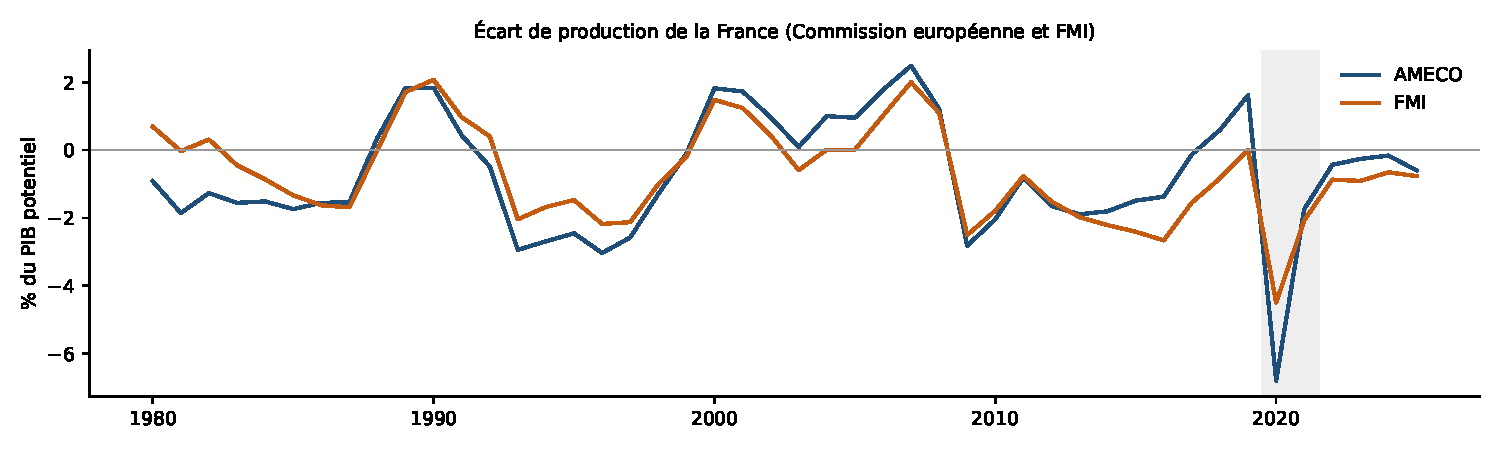
\includegraphics[width=\linewidth]{ecart_production.pdf}
\caption{Écart de production publié pour la France. L'écart est lui-même une estimation (fonction de production et
filtres) ; les deux sources divergent de 1 à 2 points certaines années.}\label{fig:ecart}
\end{figure}

\paragraph{Ce que les données identifient.} La persistance de l'écart de production : un modèle AR(2) estimé sur
1982-2019 donne φ₁ = 1,07 et φ₂ = $-0{,}30$ (AMECO), 0,98 et $-0{,}41$ (FMI). La durée moyenne d'un écart (somme de
la réponse à un écart initial de 1 sur dix ans) est de 2,8 ans (AMECO, intervalle à 90 \% : 2,0-5,3) et 2,3 ans
(FMI, 1,6-4,0).

\paragraph{Ce qu'elles n'identifient pas.} Une régression directe de l'écart sur la croissance du potentiel donne un
coefficient contemporain \emph{positif} (+3,0 avec AMECO), à l'opposé de ce qu'impliquerait un retard de la
production sur le potentiel. La raison est connue : le potentiel publié est en partie obtenu en filtrant la production
elle-même. Ce moment n'est pas utilisé.

\paragraph{Spécifications plus riches.} Une asymétrie entre phases d'expansion et de contraction (t = 0,03 et
$-0{,}47$) et une dépendance à l'état de l'économie (t = 1,4 et 1,5) ne sont pas significatives : la spécification
reste linéaire, constante dans le temps et commune aux secteurs.

\paragraph{Méthode.} Pour une grille de valeurs de ρ, θ et du terme proportionnel, le modèle complet est soumis à un
choc d'offre permanent (productivité $-1$ \% en 2028) ; on mesure la durée de l'écart de production qui en résulte. Sont
retenues les configurations dont la durée est dans l'union des intervalles à 90 \%, sans dépassement de plus de 10 \%,
et dont θ est compatible avec la réponse estimée de la consommation à un choc permanent de revenu (0,6-0,65 selon
Blundell, Pistaferri et Preston, 2008) et de l'investissement (proche de 1), soit 0,4 à 1,0.

\begin{figure}[htbp]\centering
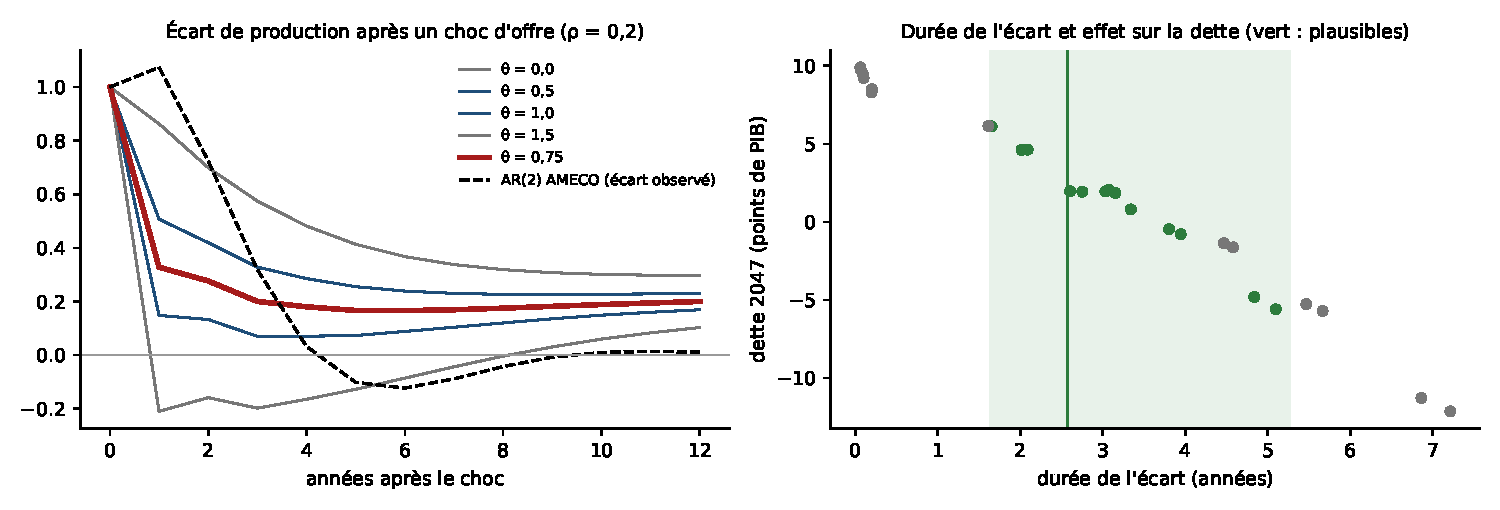
\includegraphics[width=\linewidth]{irf_theta.pdf}
\caption{À gauche : écart de production après un choc d'offre permanent selon θ (rouge : valeur retenue) et réponse de
l'AR(2) estimé sur l'écart observé. À droite : chaque point est une configuration (ρ, θ, terme proportionnel) ; en
abscisse la durée de l'écart, en ordonnée l'effet du choc sur la dette en 2047 ; la bande verte est l'intervalle
empirique.}\label{fig:irf}
\end{figure}

\begin{resultat}[Résultat de l'estimation]
Valeur centrale ρ = 0,2, θ = 0,75 (durée 3,0 ans) ; plage plausible θ de 0,5 à 1,0, ρ de 0,1 à 0,3. La valeur de la v0.7
(θ = 1,5) est rejetée : la production dépasse le nouveau potentiel de 20 à 30 \%. L'absence d'anticipation (θ = 0) est
rejetée aussi : l'écart dure de 4,6 à 7 ans. Sur toute la grille, un choc de productivité de $-1$ \% modifie la dette
de 2047 de $-12$ à +10 points selon la fermeture ; sur l'ensemble plausible, de $-6$ à +6 points. L'incertitude est
réduite, pas supprimée.
\end{resultat}

La réponse du modèle conserve une « traîne » : 15 à 20 \% de l'écart initial persiste au-delà de cinq ans, alors que
l'AR(2) observé s'annule en quatre ans. C'est une limite de la spécification (un seul terme intégral) que les données ne
permettent pas de corriger sans paramètre supplémentaire non identifié.

\section{Incidence des prélèvements sur les entreprises}

La cible de long terme du coût salarial par tête devient
\begin{equation}
\ln w^* = \ln p^{VA} + \ln \text{prod} + s_t, \qquad s_t = -\lambda_{IS}\frac{\Delta IS}{W} - \lambda_{IP}\frac{\Delta IP}{W} + (1-\lambda_{cot})\frac{\Delta \text{Cot}}{W},
\end{equation}
où $W$ est la masse salariale, λ la part supportée par les salariés (IS : 0,3 ; impôts de production : 0,2) et
$\lambda_{cot}$ la part d'une variation de cotisations employeurs transmise aux salaires (0,5). La correction d'erreur
de l'équation de salaires, estimée, donne la vitesse. Le reste de l'incidence passe par les profits (dividendes,
investissement, trésorerie) et, pour les impôts de production, par les prix.

\section{Distribution dynamique (M16)}

Pour chaque ménage $h$ et chaque horizon $t$, le revenu disponible réel après propagation est
\begin{equation}
\Delta y^{\text{réel}}_h = \frac{y_h + \sum_c \Delta y^c_h}{\exp(\Delta \ln P_h)} - y_h,
\end{equation}
où $y_h$ est le revenu disponible de l'année de base et les canaux $c$ sont : prélèvements et prestations (M10, y
compris le coût des taxes sur la consommation), salaires (variation du salaire brut par tête, nette de la variation des
cotisations employeurs, appliquée aux salaires du ménage), emploi (retours à l'emploi des chômeurs, pertes d'emploi des
salariés selon un risque relatif par âge et catégorie sociale, entrées d'inactifs ; en espérance), revenus du
patrimoine et des indépendants (variation macroéconomique répartie au prorata d'une approximation des revenus non
salariaux), droits de succession (au prorata de cette même assiette, pondérée par l'âge), indexation (pensions et
prestations suivent les prix avec un an de retard). Le déflateur $P_h$ est le prix à la consommation du modèle hors
composante fiscale (déjà comptée dans le premier canal), corrigé de la part de l'énergie dans la consommation du
décile. Chaque composante du revenu n'est modifiée que par un canal : c'est la règle contre les doubles comptes.

\section{Offre de travail (M15)}

18 cas types : 9 configurations familiales (personne seule ; parent isolé avec un ou plusieurs enfants ; couple sans
enfant, avec un ou deux enfants, avec trois enfants ou plus, chacun avec un conjoint en emploi ou sans emploi) ×
locataire ou propriétaire. L'effet d'une baisse de 10 \% des aides au logement sur la population active passe de
+72 000 à +22 000 personnes : les propriétaires, qui n'en perçoivent pas, ne sont plus comptés.

% ============================================================================================================
\chapter{Sources et calibrations}\label{ch:sources}
% ============================================================================================================

Le registre complet (définition, valeur, intervalle, source, méthode, confiance, date) est dans
\code{doc/20\_registre\_parametres\_v08.md} et dans le fichier Excel de comparaison. Les principes :
\begin{itemize}
\item une hypothèse n'est jamais présentée comme une donnée observée : chaque paramètre a un niveau de confiance
(A estimé sur données françaises, B études causales proches, C calibré sur la littérature, D hypothèse, X
exploratoire) ;
\item quand les données ne permettent pas de trancher, plusieurs valeurs sont conservées et propagées jusqu'aux
résultats (configurations « réactions faibles » et « réactions fortes », sensibilité un à un) ;
\item quand une donnée manque, la substitution et la perte de précision sont documentées.
\end{itemize}

\begin{table}[htbp]\centering\scriptsize
\caption{Paramètres modifiés ou ajoutés en v0.8.}
\begin{tabularx}{\linewidth}{@{}l r l L c@{}}\toprule
Paramètre & Valeur & Intervalle & Source & Confiance\\ \midrule
Rappel vers le potentiel ρ & 0,2 & 0,1-0,3 & Durée des écarts de production (AMECO, FMI 1982-2019) & B\\
Anticipation θ & 0,75 & 0,5-1,0 & Idem + Blundell, Pistaferri, Preston (2008) & C\\
Terme proportionnel, tensions sur les importations & 0 & 0-0,15 ; 0-0,3 & Oscillations non observées & C / D\\
Incidence salariale de l'IS & 0,3 & 0-0,5 & Fuest, Peichl, Siegloch (2018) & C\\
Incidence salariale des impôts de production & 0,2 & 0-0,4 & Hypothèse & D\\
Transmission des cotisations employeurs aux salaires & 0,5 & 0,2-1,0 & Bozio, Breda, Grenet (2019) ; Carbonnier et al. (2019) & C\\
Salaire d'embauche (M16) & 0,75 & 0,6-0,9 & Insee & C\\
Allocation perdue au retour à l'emploi (M16) & 5 200 € & 3 000-8 000 & Unédic (ordres de grandeur) & C\\
Risque relatif de perte d'emploi (M16) & âge, catégorie & — & Taux de chômage par âge et catégorie (Insee) & C\\ \bottomrule
\end{tabularx}
\end{table}

\begin{limites}[Données indisponibles]
Potentiel en temps réel publié (millésimes) ; patrimoine et héritages par ménage dans l'échantillon ; transitions
individuelles emploi-chômage (panel) ; données d'entreprises par taille appariées au modèle. Les substitutions
retenues et leur coût sont décrits dans le registre.
\end{limites}
